\chapter{Cahier de Charges}

\section*{Introduction}%
\addcontentsline{toc}{section}{\numberline{}Introduction}%
Comme son nom ce chapitre a pour but de ressortir les différents éléments présents dans le cahier de charges d’un projet. Nous allons commencer par étudier la problématique dont fait face l’entreprise et de là nous allons ressortir les objectifs du projet. Ensuite nous aborderons les besoins, les fonctionnalités et les contraintes. Puis nous allons terminer par la planification et l'estimation des couts.

\section{Contexte}
AMD est l'agent / distributeur exclusif au Cameroun de plusieurs categories de materiaux de maintenance industrielle. De ce fait la gestion commerciale est un element cle dans la survie economique de l'entreprise. AMD Sarl est une PME et comme la plupart des entreprises, pour leur aider dans la gestion de leurs activités au quotidien y compris la gestion commerciale, ils utilisent un outil de gestion commerciale en ligne, notamment l’ERP\footnote{Enterprise Resource Planning (Progiciel de Gestion Intégré en français)} Sage 100.
Cependant l'entreprise a souvent besoin d'optimiser le processus de fixation des prix de leurs produits ou encore savoir a quel moment avoir un certain produit en stock, ce qui pourrait nettement améliorer les ventes de l'entreprise. Ceci est rarement optimal. De ce fait ca devient plus difficile pour l'entreprise de fidéliser les clients ou encore acquérir des nouveaux clients. 

\section{Problématique}
\subsection{Démarche d’analyse du problème}
Pour mieux analyser notre problème, on a résolu à utiliser la méthode des 5M. Aussi appelé diagramme de causes/effets" ou "en arêtes de poisson", l'outil créé par Mr Ishikawa fait partie de ceux à posséder dans sa trousse à outils spéciale "résolution des problèmes". Rappelant le squelette d'un poisson, cet outil visuel a pour finalité de lister les causes qui ont une influence sur un effet (une situation), de les classer, de les hiérarchiser. Très utilisé par les qualiticiens, le diagramme d'Ishikawa est en fait applicable à l'ensemble des métiers de l'entreprise.
\paragraph{}
Les étapes principales dans l’utilisation de cette méthode sont les suivants :
\begin{itemize}
    \item \textbf{Qualifiez l'effet :} Il s'agit couramment du problème que vous cherchez à résoudre. Dans notre contexte on peut identifier les effets suivants :
    \begin{itemize}
        \item La diffculté à fixer un prix pouvant generer un gain maximal à un moment précis
        \item Savoir a quel moment avoir un produit en particulier en stock et la quantité pour éviter des clients insatisfaits.
    \end{itemize}
    \item \textbf{Dressez un inventaire des causes possibles }: Il s’agit de lister les causes qui ont une influence sur le problème. Dans notre contexte on peut constater que l'entreprise possède des données généres par ses systèmes de gestion qui ne sont pas exploitées. De ce fait il ya un maque d'outils pouvant aider à faire des décisions.
    \item \textbf{Classez les causes par familles :} Ici intervient les 5M qui sont fréquemment utilisés pour cette tâche : Main d’œuvre, matière, matériels, méthodes, milieu. Dans notre cas on a une seule catégorie qui est la méthode d'utilisation de nos données.
    \item \textbf{Evaluez les branches/racines qui ont le plus d'impact.}
\end{itemize}

Le diagramme Ishikawa dans la figure \ref{fig:ishikawa} nous montre l'origine des problématiques dont fait face l'entreprise.
\begin{figure}[H]
    \centering
    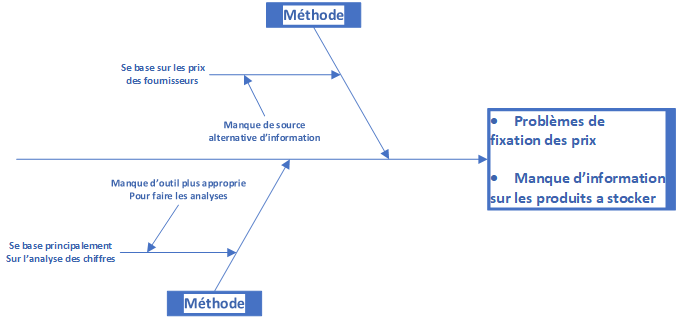
\includegraphics[width=\textwidth]{ishikawa}
    \caption{Diagramme Ishikawa analysant nos problématiques}
    \label{fig:ishikawa}
\end{figure}


\subsection{Identification de la problématique}
L’entreprise possède une quantité énorme d’informations non exploités, qui peuvent non seulement optimiser la prise de décisions par les décideurs mais aussi faciliter le travail des employés, augmentant ainsi la productivité de celles-ci, si exploitée de la bonne façon. 

De ce fait on peut identifier les difficultés  suivantes dont fait face l'entreprise, aussi représentés dans la figure 
\begin{itemize}
    \item La difficulté à fixer le prix d'un produit pour avoir un revenue maximal sur celui ci dans période bien précise.
    \item La difficulté dans l'identification des produits à mettre en stock avec les quantités à une certaine période pour éviter d'avoir des clients qui commandent des produits qu'on ne peut pas fournir.
\end{itemize}
De là on peut formuler notre problématique : \textbf{Comment fixer le prix des produits selon les périodes et savoir les besoins des clients en certaines périodes pour éviter les commandes que l'entreprise ne pourra pas satisfaire?}  



\section{Objectifs}
Après avoir posé nos problèmes, nous pouvons à présent parler des objectifs de notre projet.

\subsection{Objectif général}
L’objectif général c’est de mettre sur pied une plateforme de Business Intelligence, de l’intégration des données jusqu’à la visualisation en passant par l’analyse pour aider à la décision dans l'entreprise. 

\subsection{Objectifs spécifiques}
La solution devra nous permettre de :
\begin{itemize}
    \item Intégrer des données provenant de diverses sources notamment, l’ERP Sage 100, Gescom v14 et des fichiers Excel.
    \item Faire des analyses multidimensionnelles sur nos données.
    \item Visualiser nos données en masse et en ad hoc.
\end{itemize}


\section{Besoins}
\subsection{Besoins Fonctionnels}
Pour notre système nous recensons les besoins fonctionnels suivants :
\begin{itemize}
    \item Suivre l'évolution des ventes par période
    \item Suivre les variations de prix 
    \item Suivre les commandes et les disponibilités par période
    \item Suivre les fréquences d'indisponibilité des produits.
\end{itemize}
\subsection{Besoins Non-Fonctionnels}
Hormis les besoins fonctionnels, nous voulons un système qui nous deonnera certains assurances tels quq :
\begin{itemize}
    \item \textbf{Sécurité : }Les données ne pourront pas etre accédés par des parties non autorisés.
    \item \textbf{Robustesse : }Le système doit être stable 
    \item \textbf{Disponibilité :}On doit pouvoir accéder au système en temps et en heure
    \item \textbf{Ergonomie : }Le système doit être facile et agréable a utiliser.
\end{itemize}
\section{Fonctionnalités attendus}
De façon générale le projet a deux fonctionnalités majeures. 
\begin{itemize}
    \item \textbf{Aide a la fixation des prix des produits par période définie}
    \item \textbf{Donner des indices pour savoir quand se ravitailler pour un produit}
\end{itemize}


\section{Contraintes}
Ce projet fait face principalement à deux types de contraintes
\begin{itemize}
    \item \textbf{Les contraintes technologiques :} Ici nous parlerons technologies utilisées pour le projet. L'entreprise (prestataire) utilise déjà une suite d'outils Microsoft SSDT pour ses projets de Business Intelligence. Nous étions dont contraint d'utiliser les mêmes technologies pour notre projet.
    \item \textbf{Les contraintes temporelles :} Le temps alloué à la réalisation de ce projet était de deux mois, or le projet à été planifié sur une période de trois mois. 
\end{itemize}


\section{Intervenants du projet}
Ce projet nécessitera pour sa réalisation :
\begin{itemize}
    \item Un (01) maître d'ouvrage qui est l'entreprise cliente ;
    \item Un (01) maître d'oeuvre qui est l'analyste, concepteur et Développeur du système ;
    \item Trois (03) consultants afin de pouvoir initier, cadrer et contrôler les travaux effectués ;    
\end{itemize}

Ces ressources sont matérialisées dans le tableau suivant :
\begin{table}[H]
    \centering
    \caption{Présentation des Intervenants du projet.}
    \begin{tabular}[t]{|p{4cm}|p{7cm}|p{4cm}|}
        \hline
        \textbf{Qualité } & \textbf{Nom} & \textbf{Fonction} \\
        \hline\hline
        Maître d'ouvrage & AMD Sarl (Représente par M. KOGAING Arnold) & Porteur des besoins\\
        \hline
        Maître d'oeuvre & M. FOKOU DIFFO KANG Joel & Porteur du projet \\
        \hline
        Superviseur & Pr. AZEBAZE Anatole & Superviseur\\
        \hline
        Encadreur & M. TSAFACK Cédrique & Encadreur\\
        \hline
        Encadreur & M. DJATIO Christian & Encadreur\\
        \hline\hline
    \end{tabular}
    \label{tab:resmat}
\end{table}%



\section{Planification du projet}
Nous avons pu diviser notre projet en des grandes phases qui contiennent des tâches que nous allons représenter sur un diagramme de Gantt. Le tableau \ref{tab:gantt} recapitule ces phases et tâches.


\begin{table}[H]
    \centering
    \caption{Phases et tâches du projet.}
    \begin{tabular}[t]{|p{2cm}|p{7cm}|p{3cm}|p{3cm}|}
        \hline
        \textbf{Tâche} & \textbf{Description} & \textbf{Précédence} & \textbf{Durée (jours)} \\
        \hline\hline
        \multicolumn{4}{|c|}{\textbf{Analyse du projet}} \\
        \hline
        A & Identification du problème & - & 1 \\
        \hline
        B & Etude existant & A & 7 \\
        \hline
        C & Cahier de Charges & B & 9 \\
        \hline
        \multicolumn{4}{|c|}{\textbf{Conception}} \\
        \hline
        D & Conception DWH & C & 14 \\
        \hline
        E & Conception DM & D & 7 \\
        \hline
        F & Conception ETL & D, E & 7 \\
        \hline
        G & Documentation & B & Jusqu’à la fin \\
        \hline
        \multicolumn{4}{|c|}{\textbf{Implémentation
        }} \\
        \hline
        H & Installation Outils & F & 2 \\
        \hline
        I & Construction DWH & H & 2 \\
        \hline
        J & Construction DM & I & 2 \\
        \hline
        K & Construction ETL & I, J & 3 \\
        \hline
        L & Alimentation DWH & K & 2 \\
        \hline
        M & Alimentaion DM & K & 2 \\
        \hline
        N & Construction cubes & M & 14 \\
        \hline
        O & Construction TDB & M, N & 14 \\
        \hline
        \multicolumn{4}{|c|}{\textbf{Déploiement}} \\
        \hline
        P & Déploiement & N & Jusqu’à la fin \\
        \hline
        Q & Test & P & Jusqu’à la fin \\
        \hline\hline

    \end{tabular}
    \label{tab:gantt}
\end{table}%


La figure \ref{fig:gantt} représente le diagramme de Gantt du projet.


\begin{figure}[H]
    \centering
    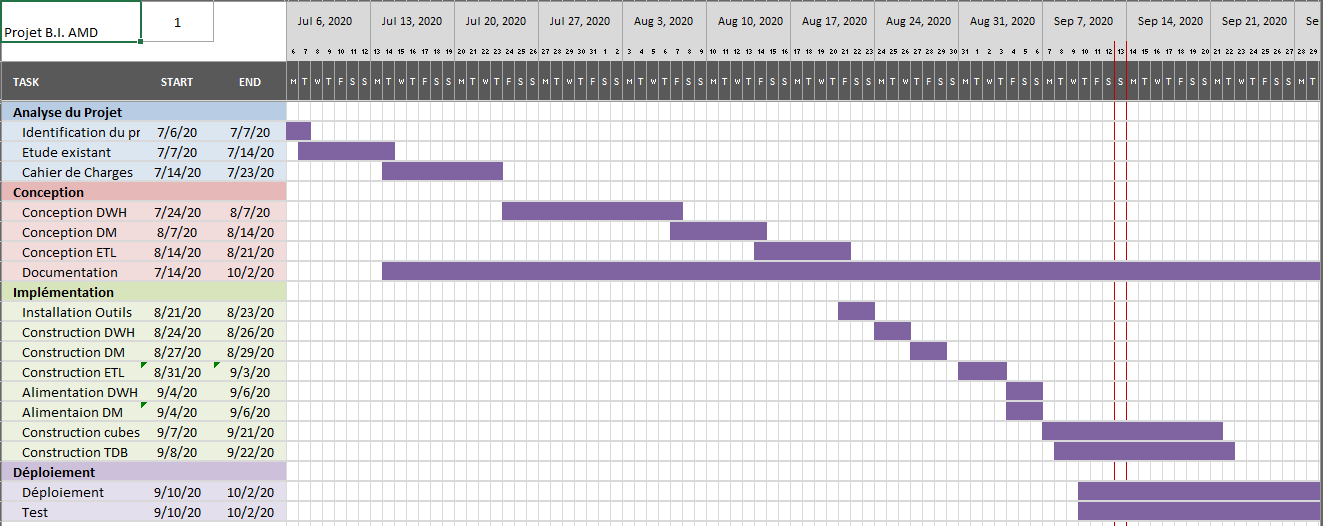
\includegraphics[width=\textwidth]{gantt}
    \caption{Diagramme de Gantt.}
    \label{fig:gantt}
\end{figure}


\section{Estimation des coûts}
\subsection{Méthode d’estimation des coûts}
Afin d’évaluer le coût de notre projet, on doit d’abord définir les éléments de base qui constituent notre projet : 
\begin{itemize}
    \item Le planning initial du projet
    \item La durée de chaque tâche
    \item La durée totale du projet
    \item Les ressources humaines nécessaires
    \item Les ressources matérielles nécessaires
    \item Les ressources logiciels nécessaires
\end{itemize}

On distingue deux méthodes d’estimation des coûts :
\subsubsection{La méthode analogique}
Cette méthode consiste à se référer aux coûts réels des projets similaires au vôtre et à les adapter en faisant quelques ajustements. Il est également possible de s’appuyer sur l’avis d’un chef de projet expérimenté qui a travaillé sur un projet semblable. Elle se déroule en trois étapes :
\begin{itemize}
    \item Analyse du projet ;
    \item Recherche d’un projet similaire ;
    \item Comparaison et chiffrage.
\end{itemize}

\subsubsection{La méthode ascendante}
Le but de cette méthode est d’estimer le coût de chaque groupement de tâches, puis d’additionner chacune de ces estimations afin d’obtenir le coût global du projet. Cette méthode est plus précise que la précédente car elle s’appuie sur l’expérience et l’avis des personnes qui exécutent les tâches en question. Cette méthode s’utilise lors de l’élaboration du budget. Une fois que tous les éléments du projet ont été chiffrés, on les additionne afin d’obtenir le coût total du projet.


Nous optons pour la deuxième méthode, \textbf{la méthode ascendante} pour plus de précision.

\subsection{Coût du Projet}
\begin{table}[H]
    \centering
    \caption{Coût de ressources matérielles.}
    \begin{tabular}[t]{|p{3cm}|p{4cm}|p{2cm}|p{3cm}|p{3cm}|}
        \hline
        \textbf{Ressource} & \textbf{Caractéristiques} & \textbf{Quantité} & \textbf{Coût Unitaire} & \textbf{Coût Total}\\
        \hline\hline
        Ordinateur portable & Toshiba (i3-1.9GHz), Mémoire vive: 8GB & 01 & 200 000 FCFA & 200 000 FCFA\\
        \hline\hline
    \end{tabular}
    \label{tab:resmat}
\end{table}%

Dans le tableau \ref{tab:reshum} qui représente l'estimation des couts humaines pour le projet, on s'est basé sur la moyenne de salaires d'un developpeur de Business Intelligence au Cameroun pour estimer le prix d'une journée de travail de celui ci. Ceci nous a mené a la somme de \textbf{20 000 FCFA} par journée de travail. Et en se basant sur la méthode ascendante d'estimation des coûts on obtient le suivant.

\begin{table}[H]
    \centering
    \caption{Coûts des ressources humaines.}
    \begin{tabular}[t]{|p{2cm}|p{1.5cm}|p{3cm}|p{1.5cm}|p{3cm}|p{3cm}|} 
        \hline
        \textbf{Ressource} & \textbf{Nombre} & \textbf{Nom} & \textbf{Durée (jours)} & \textbf{Coût Unitaire} & \textbf{Coût Total}\\
        \hline\hline
        Analyste-Concepteur & 01 & FOKOU DIFFO KANG Joel & 34 & 20 000 FCFA & 680 000 FCFA\\
        \hline
        Développeur B.I. & 01 & FOKOU DIFFO KANG Joel & 31 & 20 000 FCFA & 620 000 FCFA\\
        \hline
        \textbf{Total} & \multicolumn{5}{c|}{1 300 000 FCFA} \\
        \hline\hline
    \end{tabular}
    \label{tab:reshum}
\end{table}%


\begin{table}[H]
    \centering
    \caption{Coût total de développement.}
    \begin{tabular}[t]{|p{8cm}|p{7.5cm}|} 
        \hline
        \textbf{Ressource} & \textbf{Coût} \\
        \hline\hline
        Ressources Matérielles & 200 000 FCFA \\
        \hline
        Ressources Humaines & 1 300 000 FCFA \\
        \hline
        \textbf{Coût Total de développement} & \textbf{1 500 000 FCFA} \\
        \hline\hline
    \end{tabular}
    \label{tab:couttotal}
\end{table}%



\section*{Conclusion}%
\addcontentsline{toc}{section}{\numberline{}Conclusion}% 
Dans ce chapitre il était question de ressortir les éléments du cahier de charges et présenter les besoins. Nous avons terminé avec une planification et une estimation des couts du projet.